\section{Evaluation Metrics}
\label{sec:evaluation_metrics}
Evaluation is usually referred as estimating the performance of a system under test
when confronted with new data. For an objective evaluation, the system is fed
previously unseen data for which reference annotations are available. The system output is then compared to the reference to calculate measures of its performance.

What performance means and how it should be measured may vary depending
on the specifications and requirements of the developed system: We can measure
accuracy to reflect how often the system correctly classifies or detects a sound, or we can measure error rates to reflect how often the system makes mistakes. By using
the same data and the same methodology to evaluate different systems, a fair and direct comparison can be made of systems’ capabilities.

The metrics used in detection and classification of sound events include accuracy, precision, recall, F-scor, area under the curve (AUC) or error rate (ER). There is no metric universally good for every kind of algorithm, as they each reflect different perspectives on the ability of the system.

\subsection{Metrics Computation}
Basically, the evaluation metrics are computed by comparing the prediction of the system under analysis with the respective annotations or \textit{ground truth}. Thus, the metrics are calculated based on counts of the correct predictions and different types of errors made by the system.
These counts are referred to as intermediate statistics and are defined depending on the evaluation procedure. These intermediate statistics are defined as follows for a target sound event:

\begin{itemize}
	\item True positive: A correct prediction, meaning that the system output and the reference both indicate the event present.
	\item True negative: The system output and the reference both indicate event not present.
	\item False positive: The system output indicates event  present or active, while the reference indicates event not present.
	\item False negative: The system output indicates event not present or inactive, while the reference indicatesit as present.
\end{itemize}

Sound event classification is usually a single-label multiclass problem, and the resulting intermediate metrics reflect whether the single true class is correctly recognized for each example. In this task there is no distinction between false positives and false negatives. 
In sound event detection, the choice of measurement determines the interpretation of the result: With a segment-based metric, the performance shows how well the system correctly detects the temporal regions where a sound event is
active; with an event-based metric, the performance shows how well the system is able to detect event instances with correct onset and offset. Thus, in the segment-based metric the ground truth and system output are compared in a fixed time grid, and sound events are marked as active or inactive in each segment. For the event-based metric the ground truth and system output are compared at event instance level. Specifically, the intermediate statistics for sound event detection are defined as follows:

\begin{itemize}	
	\item Substitutions $S$: are the number of ground truth events for which we have a false positive and one false negative in the same segment; %, thus: $S(t_1) = \min(FN(t_1),FP(t_1))$;	
	\item Insertions $I$: are events in system output that are not present in the ground truth, thus the false positives which cannot be counted as substitutions;%: $I(t_1) = \max(0,FN(t_1)-FP(t_1))$;
	
	\item Deletions $D$: are events in ground truth that are not correctly detected by the system, thus the false negatives which cannot be counted as substitutions;%: $D(t_1)= \max(0,FP(t_1)-FN(t_1))$.	
\end{itemize}

If we consider the scenario of polyphonic sound event detection, the segment-based metric essentially
splits the duration of the test audio into fixed length segments that have multiple associated labels, reflecting the sound events active anywhere in the given segment. In this respect, evaluation verifies if the system output and reference coincide in the assigned labels, and the length of the segment determines the temporal resolution of the evaluation. 
Event-based metrics compare event instances one to one. Since the time extents of the events detected by the system may not exactly match the ground truth, a common approach is to allow a time misalignment threshold or \textit{time-collar}.

\subsubsection{Performance Metrics}
Measures of performance are calculated based on accumulated values of the intermediate statistics. 
We denote by $TP$, $TN$, $FP$, and $FN$ the sums of the true positives, true negatives, false positives, and false negatives accumulated throughout the test data. In the case of multiclass problem, the accumulation of intermediate statistics can be performed either globally or separately for each class, depending on the nature of the problem (i.e., instance-based or class-based) or datasets characteristics (i.e., highly unbalanced classes).
Based on the total counts of the intermediate statistics, many different measures can be derived.  We can define:

\begin{eqnarray}
\text{Accuracy} =& \frac{TP+TN}{TP+TN+FP+FN} \\
\text{Precision} =& \frac{TP}{TP+FP} \\
\text{Recall} =& \frac{TP}{TP+FN}  \\
\text{F-score} =& \frac{2TP}{2TP+FN+FP}  
\end{eqnarray}

Accuracy measures how often the classifier makes the correct decision,
 as the ratio of correct system outputs to total number of outputs. Precision, recall, and F-score were introduced in the context of information retrieval. F-score can be also calculated as the harmonic mean of Precision and Recall scores:

\begin{equation}
 \text{F-score} = 2 \cdot \frac{\text{Precision}\cdot\text{Recall}}{\text{Precision}+\text{Recall}}
\end{equation}

F-score has the advantage of being a familiar and well understood metric. Its main drawback is that its value is strongly influenced by the choice of averaging and the data balance between classes: in instance-based averaging the performance
on common classes dominates, while in class-based averaging (balanced metrics) it is necessary to at least ensure presence of all classes in all folds in the test data, to avoid cases when recall is undefined.

In the case of sound event detection systems, Error Rate score is the most common evaluation metric. Considering a single time frame  $t_1$, the ER is computed from its intermediate statistics, i.e., the number of substitutions ($S(t_1)$), insertions ($I(t_1)$), deletions ($D(t_1)$) and active sound events from annotations ($N(t_1)$). Formally, for the entire evaluation set:

\begin{equation}
ER = \frac{\sum_{t_1=1}^{T} S(t_1) + \sum_{t_1=1}^{T} I(t_1) + \sum_{t_1=1}^{T} D(t_1)}{\sum_{t_1=1}^{T} N(t_1)},
\end{equation}
where $T$ is the total number of segments $t_1$.


\subsection{Detection Metrics}
Precision and recall rely on hard decisions made for each trial, they typically depend on a threshold applied to some underlying decision variable, i.e., the output of the neural network. 
Lowering the threshold will increase likelihood of accepting both positive and negative examples, improving recall but in many cases hurting precision. Although F-score combines these values at a single threshold in an attempt to balance this
tradeoff, a more complete analysis can be provided by plotting a function proportional to the metric over the full range of possible thresholds. Some examples are, the precision-recall (P-R) curve (showed in \figref{fig:roc}) and the receiver operating characteristic (ROC) curve. The latter plots true positive rate (TPR = $TP/TP+FN$) as a function of the false
positive rate (FPR = 1 - Recall) as the decision threshold is
varied. 

These curves carry rich information, they can be difficult to compare, so a
 single figure of merit summarizing the tradeoff is desirable. The
relative ``compressed'' scores for P-R and ROC curve are respectively Average Precision (AP) score
or Area under curve (AUC), defined as:

\begin{equation}
\text{AP} = \sum_n (R_n-R_{n-1})P_n,
\end{equation}
where $R_n$ and $P_n$ are the Recall and Precision for threshold $n$ respectively and
\begin{equation}
\text{AUC}=\int _{\infty }^{-\infty }{\mbox{TPR}}(T){\mbox{FPR}}'(T)\,dT
\end{equation}
Both AUC and AP vary between 0 and 1, with an uninformative classifier yielding 0.5, while the ideal system yelds 1.


\begin{figure}[h]
	\centering
	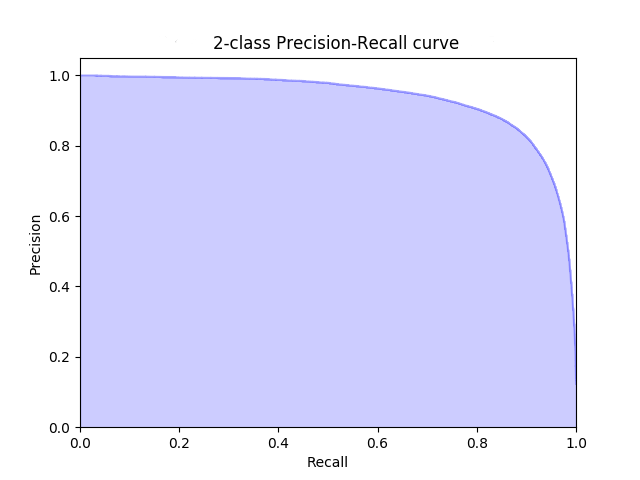
\includegraphics[width=0.5\linewidth]{img/precision_recall_curve.png}
	\caption[P-R Curve]{Example of 2-class Precision-Recall curve. Relative AP is equal to 0.9341.}	
	\label{fig:roc}
\end{figure}

\subsection{Final Remarks}
Estimates of metrics on classes with very few examples are also intrinsically noisy. Any dataset of real-world
recordings will most likely have unbalanced event classes; therefore, the experiment setup must be built with the choice of metric in mind. In a cross-validation approach, a more stable result is given by treating the cross-validation folds as single experiment, meaning that metrics are calculated only after training and testing all folds, not as average of the individual folds nor as average of individual class performance. In addition, reporting the variance among the individual folds’ contributions to the average
can serve as a useful confidence interval.
Anyway, if there are multiple scenes in the dataset, typically evaluation metrics are calculated for each scene separately and then the results are presented as the average across the scenes.


Attention should be also paid to statistical significance of the results and it should be used to calculate the theoretical limits of discriminability of the evaluation, especially when two methods/approaches/techniques are compared.


A detailed and visualized explanation of evaluation score in multi label setting for sound event analysis can be found in  \cite{mesaros2016metrics}.







%In this work we used the Error Rate (ER) as primary evaluation metric to ensure comparability with the reference systems. In particular, for the evaluations on the TUT-SED 2016 and 2017 datasets we consider a segment-based ER with a one-second segment length, while for the TUT-Rare 2017 the evaluation metric is event-based error rate calculated using onset-only condition with a collar of 500 ms. 
%

